\documentclass[a4paper]{article}
\usepackage[top=1in, bottom=1.25in, left=1.25in, right=1.25in]{geometry}
\usepackage{amsmath}
\usepackage{multicol}
\usepackage{graphicx}
\usepackage[utf8]{inputenc}
\usepackage[english]{babel}
\setlength{\parskip}{0.03cm plus4mm minus3mm}
\RequirePackage{ltxcmds}[2010/12/07]
%opening
\title{Binary Source}

\begin{document}

\maketitle
This block generates a sequence of binary values (1 or 0) and it can work in four different modes: 

\begin{multicols}{2}
\begin{enumerate}
	\item Random
	\item PseudoRandom 
	\item DeterministicCyclic 
	\item DeterministicAppendZeros 
\end{enumerate}
\end{multicols}

\subsection*{Input Parameters}

\begin{multicols}{2}
	\begin{itemize}
		\item mode
		\item probabilityOfZero 
		\item patternLength 
		\item bitStream 
		\item numberOfBits 
		\item bitPeriod 
	\end{itemize}
\end{multicols}

\subsection*{Functional description}

The \textit{mode} parameter can take integer values from 1 to 4 (that correspond, respectively, to Random, PseudoRandom, DeterministCyclic and DeterministAppendZeros modes) and allows the user to select between one of the four operation modes of the binary source.

\subparagraph*{Random Mode}
Generates a 0 with probability \textit{probabilityOfZero} and a 1 with probability 1-\textit{probabilityOfZero}.

\subparagraph*{Pseudorandom Mode} 
Generates a pseudorandom sequence with period $2^\textit{patternLength}-1$.

\subparagraph*{DeterministicCyclic Mode}
Generates the sequence of 0's and 1's specified by \textit{bitStream} and then repeats it.

\subparagraph*{DeterministicAppendZeros Mode}
Generates the sequence of 0's and 1's specified by \textit{bitStream} and then it fills the rest of the buffer space with zeros.

\subsection*{Input Signals}

(Currently working with no input signal.)

\subparagraph*{Number:} 0 or 1 (which would work as a trigger)

\subparagraph*{Type:} Binary (DiscreteTimeDiscreteAmplitude)

\subsection*{Output Signals}

\subparagraph*{Number:} 1 or more

\subparagraph*{Type:} Binary (DiscreteTimeDiscreteAmplitude)

\subsection*{Examples} 

\paragraph*{Random Mode}

\paragraph*{PseudoRandom Mode}
As an example consider a pseudorandom sequence with \textit{patternLength}=3 which contains a total of 7 ($2^3-1$) bits. In this sequence it is possible to find every combination of 0's and 1's that compose a 3 bit long subsequence with the exception of $000$. For this example the possible subsequences are $100$, $010$, $001$, $110$, $101$, $011$ and $111$. Some of these require wrap. 

\begin{center}
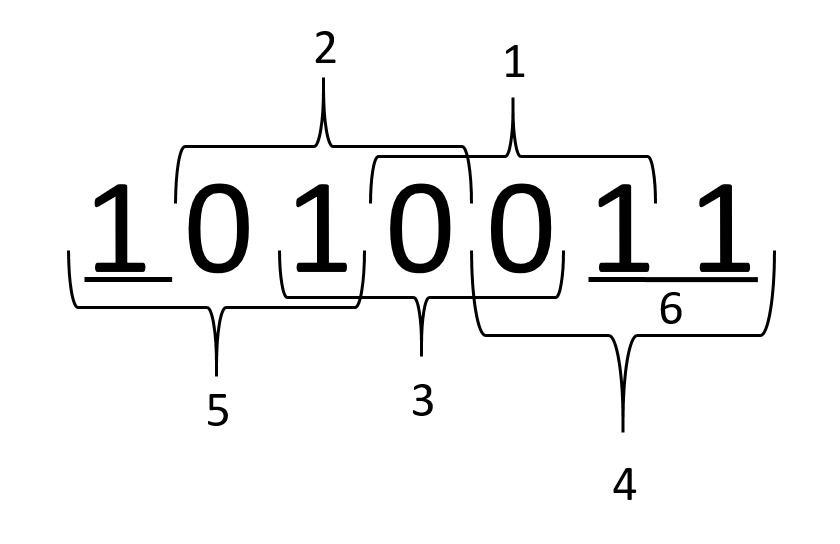
\includegraphics[width=0.5\textwidth]{BinarySequenceN3}
\end{center}

\paragraph*{DeterministicCyclic Mode}

\paragraph*{DeterministicAppendZeros Mode}

\subsection*{Sugestions for future improvement}

Implement an input signal that can work as trigger.

\end{document}